\documentclass{beamer}
\usetheme{CambridgeUS}
\usecolortheme{rose}

%\usebackgroundtemplate
%{
%	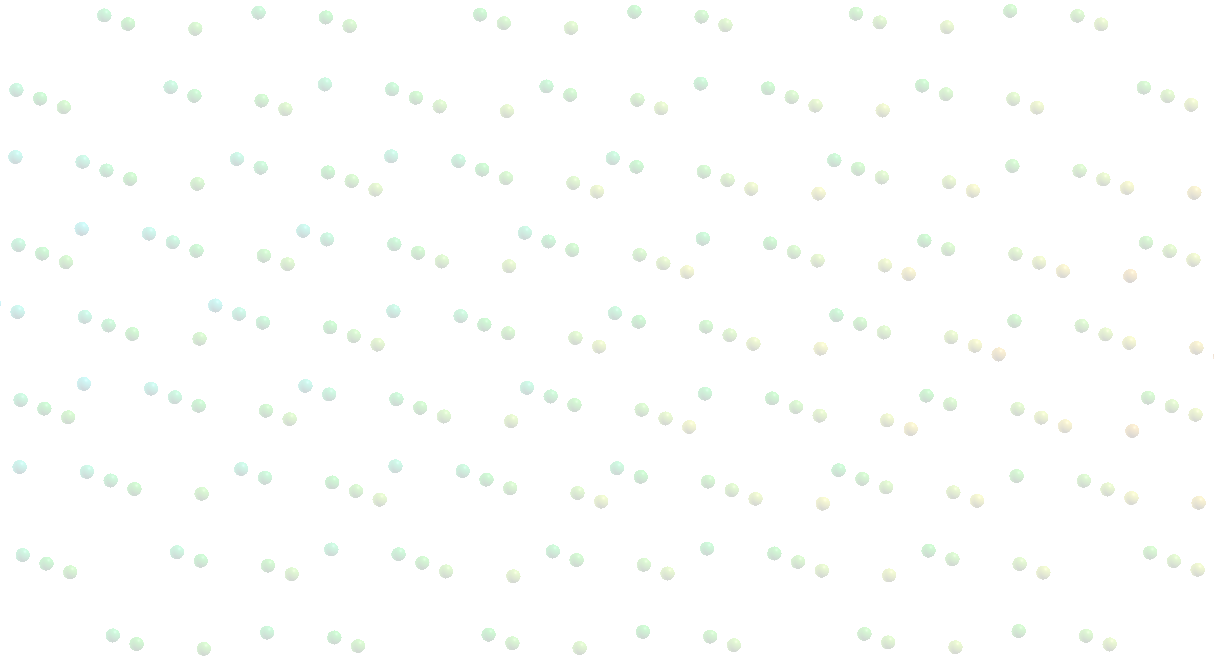
\includegraphics[width=\paperwidth,height=\paperheight]{r9coloured.png}
%}


\title{Computing P‐T Diagrams from First Principles}
\author{Max Tyler}
\institute{The University of Edinburgh}
\date{\today}
 
 
 
\begin{document}
 
\frame{\titlepage}
 
\begin{frame}
	\frametitle{What's this About?}
\end{frame}

\begin{frame}
	\frametitle{What is DFT?}
\end{frame}

\begin{frame}
	\frametitle{How to recreate the P-T diagram of Na?}
\end{frame}

\begin{frame}
	\frametitle{Lithium Paper}
\end{frame}
 
\begin{frame}
	\frametitle{Silicon}
\end{frame}

\begin{frame}
	\frametitle{Tin}
\end{frame}

\begin{frame}
	\frametitle{Sodium}
\end{frame}

\begin{frame}
	\frametitle{Not 9R Any More!}
\end{frame}

\begin{frame}
	\frametitle{Further Research}
	Look into other phases in this region (HCP, etc.)
\end{frame}

\end{document}

